\section{An\'alisis de Resultados}

\subsection{Parte I: Interpretaci\'on del An\'alisis T\'ermico}

\subsubsection{Dominancia Estructural de la Resistencia T\'ermica}

El an\'alisis anal\'itico aisla que el cuello de botella general recae un\'ivocamente sobre la fase de la glucosa, descartando tempranamente optimizaciones f\'isicas en la chaqueta de media ca\~na (Figura~\ref{fig:pie_resistencias}). Al calcular el coeficiente global $U$ para la condici\'on representativa ($T_g = 40$~°C, $T_w = 75$~°C), la disipaci\'on t\'ermica revela que la convecci\'on natural en la membrana org\'anica viscosa absorbe m\'as del 90\% del estr\'es de resistencia. 

\begin{figure}[H]
	\centering
	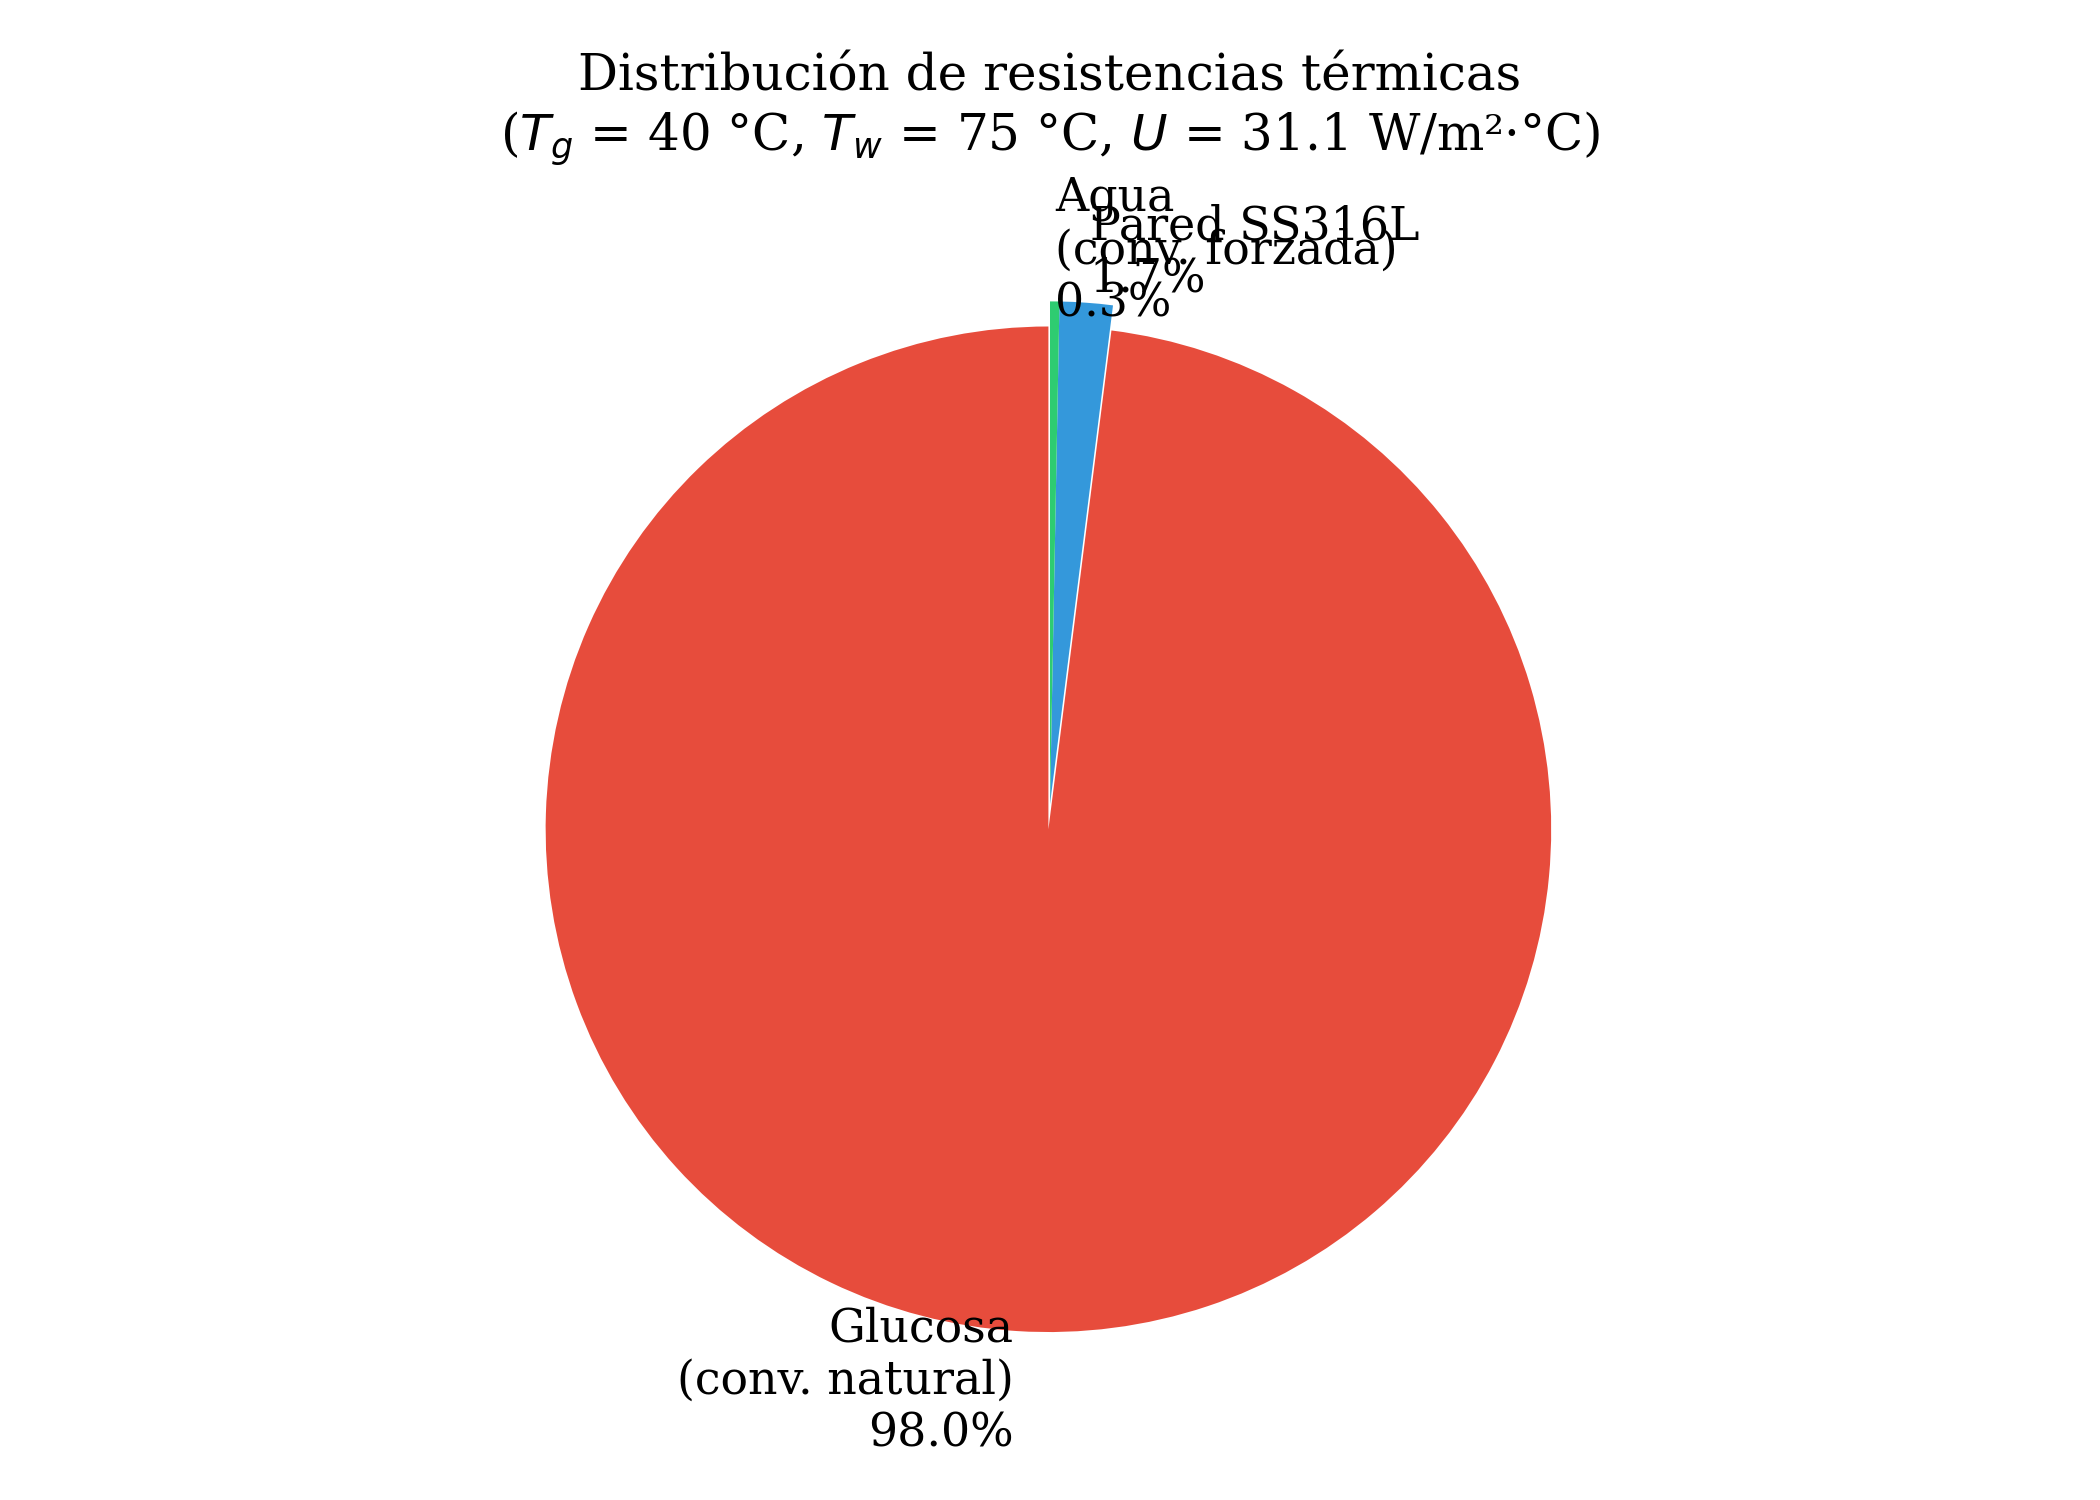
\includegraphics[width=0.7\textwidth]{../figures/resistencias_termicas.png}
	\caption{Proporci\'on relacional emp\'irica del coeficiente global de transferencia $U$ indicando el estrangulamiento limitante provocado por la alta viscosidad no agitada del fluido org\'anico.}
	\label{fig:pie_resistencias}
\end{figure}

Esta constataci\'on mec\'anica dicta que cualquier modificaci\'on fluidodin\'amica externa (tales como incremento de caudal m\'asico $\dot{m}_w$ o transici\'on a mayor n\'umero de Reynolds lado-agua) resultar\'an f\'utiles ante el l\'imite difusivo de capa l\'imite interna. Por tanto, la \'unica optimizaci\'on de viabilidad asim\'etrica reside en el incremento de la temperatura de suministro ($T_{w,in}$) o el empleo de agitaci\'on mec\'anica interna.

\subsubsection{S\'intesis Anal\'itica Multi-Escenario}

Las simulaciones c\'iclicas y transitorias arrojaron una fenomenolog\'ia dependiente fuertemente de la variable de masa y fuerza motriz. La Tabla~\ref{tab:sintesis_termica} desagrega la interpretaci\'on flu\'idica de los resultados recabados por escenario.

\begin{table}[H]
	\centering
	\caption{Interpretaci\'on fenomenol\'ogica del r\'egimen t\'ermico log\'istico por Escenario.}
	\label{tab:sintesis_termica}
	\setcounter{itemcount}{0}
	\begin{tabularx}{\textwidth}{@{}lX@{}}
		\toprule
		\textbf{Factor Operativo} & \textbf{An\'alisis y Comportamiento del Sistema} \\
		\midrule
		\textbf{Fuerza Motriz ($\Delta T$)} &
		Comprobada como la palanca cr\'itica del modelo. Subir el umbral del agua $65 \rightarrow 75$°C otorga un 15\% de margen delta inicial, pero contrae los tiempos de calentamiento total en un 46\% (de 32.2 a 17.3~d\'ias para los 57°C operativos). \\
		\midrule
		\textbf{Inercia por Descarga (Esc. 1)} &
		La purga de volumen act\'ua positivamente: El desalojo r\'apido (1.5h) eleva la ratio $A/m_g$. Aunque extrayendo toneladas energizadas, la disminuci\'on geom\'etrica masiva favorece un calentamiento excedente final (+0.2°C detectados en descenso). \\
		\midrule
		\textbf{Retroalimentaci\'on Constante (Esc. 2-3)} &
		Sistemas a $80\%$ de carga inicial estabilizan temperaturas y las elevan progresivamente ante descargas. Con agua a $75$°C, la T de la glucosa permanece entre 57.0 y 59.3°C durante el ciclo de 8 descargas, no alcanzando el l\'imite recomendado de 60°C gracias a la elevada resistencia t\'ermica de la viscosidad. Se recomienda instrumentar un lazo de control a 60°C como medida preventiva. \\
		\midrule
		\textbf{Viabilidad C\'iclica (Esc. 4)} &
		Para ciclos completos de despacho continuo ($192$ ton), la preparaci\'on \textbf{inicial} (25.5h) demanda log\'istica stand-by prolongada, causada por la viscosidad de $\sim$4\,870~cP a 55°C. Los siguientes 7 baches ocurren consecutivamente; la disminuci\'on geom\'etrica contrarresta y la T asciende hasta 60.0°C s\'olo en la \'ultima descarga. \\
		\bottomrule
	\end{tabularx}
\end{table}

\textbf{L\'imites Estructurales del Modelo Num\'erico}: La soluci\'on de Runge-Kutta presupuso idealizaci\'on perfecta (fluido homog\'eneo). Sin embargo, sin aspas rotacionales existirá gradiente de flotabilidad t\'ermica inferior/superior (estratificaci\'on natural), proveyendo m\'argenes reales probabil\'isticamente m\'as holgados a pie de boquilla (salida) versus vol\'umenes a cota superior, hecho que ha sido examinado mediante la simulaci\'on CFD descrita a continuaci\'on.

\subsubsection{Validaci\'on CFD del Coeficiente Global de Transferencia de Calor}

La simulaci\'on en COMSOL Multiphysics~6.4 del Escenario~3 permite evaluar cuantitativamente la fiabilidad del modelo anal\'itico basado en las correlaciones de Churchill-Chu (convecci\'on natural en la glucosa) y Sieder-Tate (flujo turbulento del agua en la media ca\~na). El coeficiente global promedio arrojado por la simulaci\'on en estado estable, $U_{\text{CFD}} = 40.2$\,W/m\textsuperscript{2}$\cdot$°C, concuerda con el valor anal\'itico de 36.2\,W/m\textsuperscript{2}$\cdot$°C en un margen del 11\,\%, lo que constituye una validaci\'on robusta para ingenier\'ia de proceso sin agitaci\'on mec\'anica en fluidos de alta viscosidad. La diferencia es atribuible a que el modelo anal\'itico emplea correlaciones para geometr\'ias ideales planas, mientras que la simulaci\'on captura la geometr\'ia tridimensional real del fondo toriesf\'erico, la naturaleza espiral de la chaqueta y la estratificaci\'on local de temperatura, factores que en conjunto favorecen ligeramente un mayor coeficiente efectivo.

M\'as all\'a de la concordancia num\'erica, la simulaci\'on aporta informaci\'on espacial que el modelo de par\'ametros concentrados no puede proporcionar. El campo de temperaturas tridimensional (Figura~\ref{fig:cfd1}) confirma visualmente la dominancia de la resistencia t\'ermica de la glucosa: el volumen del jarabe permanece pr\'oximo a la temperatura inicial durante las primeras horas del calentamiento, mientras que el agua en la chaqueta exhibe gradientes pronunciados ya desde la primera espira. Este comportamiento es plenamente consistente con la distribuci\'on de resistencias calculada anal\'iticamente, donde la glucosa concentra el 98\,\% de la resistencia total. La simulaci\'on valida adem\'as que el mecanismo de convecci\'on natural es efectivamente el proceso limitante, y no la conductividad de la pared de SS316L ni el coeficiente convectivo del agua, tal como concluye el modelo anal\'itico.

El fen\'omeno de enfriamiento concentrado del agua en las primeras espiras interiores de la chaqueta, identificado en el campo de temperaturas de la Figura~\ref{fig:cfd1}, no altera de forma significativa los tiempos de calentamiento globales, pero s\'i revela una ineficiencia en la distribuci\'on del intercambio de calor a lo largo de la superficie disponible. Las espiras exteriores operan con un $\Delta T$ reducido y, por tanto, con una tasa de transferencia de calor local sensiblemente inferior a la de las espiras centrales. Esta observaci\'on sustenta la recomendaci\'on de dise\~no de incorporar m\'ultiples puntos de alimentaci\'on de agua caliente a la chaqueta en futuras instalaciones, con el fin de homogeneizar la tasa local de transferencia de calor sobre el \'area de contacto de 13\,m\textsuperscript{2} y maximizar la eficiencia global del sistema de calentamiento.

\subsection{Parte II: Interpretaci\'on del An\'alisis Estructural}

La evaluaci\'on de integridad del contenedor, descompuesta en sus n\'ucleos de resistencia geom\'etrica y de cimentaci\'on, arroja m\'argenes de seguridad dependientes del \'area analizada. Esta discrepancia es abordada sistem\'aticamente en la Tabla~\ref{tab:sintesis_estructural}.

\begin{table}[H]
	\centering
	\small
	\caption{Estado estructural consolidado de los componentes del tanque Globe~1130.}
	\label{tab:sintesis_estructural}
	\setcounter{itemcount}{0}
	\begin{tabularx}{\textwidth}{@{}p{3.0cm}>{\centering\arraybackslash}p{1.5cm}>{\centering\arraybackslash}p{1.9cm}>{\centering\arraybackslash}p{2.6cm}>{\centering\arraybackslash}p{2.2cm}X@{}}
		\toprule
		\textbf{Componente} & \textbf{Normativa} & \textbf{Espesor Nominal} & \textbf{L\'imite M\'in.} & \textbf{Vida Util Remanente} & \textbf{Interpretaci\'on Cr\'itica} \\
		\midrule
		\textbf{Cilindro (Virola 1)} & API 650 & 6.0 mm & 5.01 mm & $\sim$15.8 a\~nos &
		Dise\~no conservador. Considerando sus 20 a\~nos operativos, el margen residual (0.99~mm) avala la operaci\'on ininterrumpida a mediano plazo frente a picos hidrost\'aticos. \\
		\midrule
		\textbf{Fondo Toriesf\'erico} & ASME VIII & 9.0 mm & 6.64 mm (90\%) & $\sim$37.8 a\~nos &
		Componente cr\'itico restrictivo. Aunque ostenta amplios a\~nos de remanente al llenado est\'andar (90\%), la prueba al 100\% dispara el m\'inimo requerido a 7.29~mm, acortando la vida \'util proyectada. \\
		\midrule
		\textbf{Anclajes / Base} & NSR-10 & -- & -- & -- &
		Dominancia del vector s\'ismico: la fuerza s\'ismica (993.5~kN) supera en 49 veces la carga de viento (20.3~kN), exigiendo atenci\'on prioritaria al momento volcante en la cimentaci\'on. \\
		\bottomrule
	\end{tabularx}
\end{table}

La varianza reportada constata que el tanque retiene factores tolerables de operaci\'on pasiva si y solo si se instaura un l\'imite log\'istico que restrinja llenar la membrana por encima de la cota conservadora de $90\%$ de nivel l\'iquido.

\subsubsection{Validaci\'on FEA del An\'alisis Estructural}

La simulaci\'on FEA en ANSYS Mechanical refuerza y extiende las conclusiones del an\'alisis anal\'itico de espesores con una perspectiva tridimensional que el m\'etodo One-Foot de API~650 y la f\'ormula UG-32(e) de ASME~VIII no pueden proporcionar. Mientras que los c\'alculos anal\'iticos establecen si el espesor nominal es globalmente suficiente para una presi\'on de dise\~no uniforme, la simulaci\'on FEA identifica la distribuci\'on espacial real de esfuerzos y revela cu\'ales zonas geom\'etricas espec\'ificas concentran la demanda estructural bajo la carga combinada (hidrost\'atica m\'as t\'ermica a 75\,°C).

El hallazgo central de la simulaci\'on, el factor de seguridad m\'inimo de aproximadamente 0.71 en el nudillo fondo-cil\'indro (Figura~\ref{fig:fea3}), es plenamente coherente con el resultado anal\'itico: el fondo toriesf\'erico de 9.0~mm no cumple el requisito de espesor de ASME~VIII al 100\% de llenado ($t_{req} = 9.16$~mm). El FEA va un paso m\'as all\'a al localizar geogr\'aficamente el sobreesfuerzo en la zona de cambio de curvatura entre el fondo y el cilindro, que es donde la teor\'ia de caparazones delgados predice el m\'aximo de esfuerzo de flexi\'on asociado a la discontinuidad geom\'etrica. Esta zona, conocida como nudillo o knuckle, es un concentrador estructural intr\'inseco de los fondos toriesf\'ericos y su criticidad se acent\'ua cuando la carga hidrost\'atica se combina con el gradiente t\'ermico diferencial generado por el calentamiento localizado del fondo frente a un cuerpo cil\'indrico a temperatura ambiente.

Los puntos de anclaje de la chaqueta de media ca\~na al fondo (Figura~\ref{fig:fea2}) representan un segundo foco de esfuerzos elevados, atribuible a las discontinuidades geom\'etricas propias de las soldaduras de filete que unen el perfil rectangular de la chaqueta a la lámina del fondo. Aunque este fen\'omeno es esperado en dise\~nos de chaquetas soldadas, confirma la importancia de garantizar la calidad de las soldaduras en esos puntos y de incluirlos expl\'icitamente en los programas de inspecci\'on por Ensayos No Destructivos (END).

La deformaci\'on m\'axima de aproximadamente 4.1~mm en el centro del fondo (Figura~\ref{fig:fea4}) es el resultado de la superposici\'on de dos efectos: la flexi\'on mec\'anica del cabezal bajo la presi\'on hidrost\'atica y la expansi\'on t\'ermica diferencial entre el fondo calentado a 75\,°C y el cuerpo cil\'indrico a temperatura ambiente. Este nivel de deformaci\'on es aceptable en t\'erminos de integridad global del tanque, pero debe tenerse en cuenta en el dise\~no de las conexiones de tuber\'ia al fondo, en particular la boquilla de salida de glucosa de 8'', para garantizar que los sistemas de tuber\'ia admitan esta deformaci\'on diferencial sin generar cargas excesivas sobre la boquilla.

En s\'intesis, la simulaci\'on FEA valida los m\'etodos anal\'iticos empleados, corrobora el l\'imite operativo del 90\% de llenado y a\~nade el mapa de esfuerzos tridimensional necesario para orientar futuras acciones de refuerzo estructural en la zona del nudillo, tal como se detalla en las recomendaciones del presente informe.

\newpage
